\documentclass{article}
\usepackage{tikz}
\usetikzlibrary{arrows.meta}

\begin{document}

\begin{figure}[htbp]
  \centering
  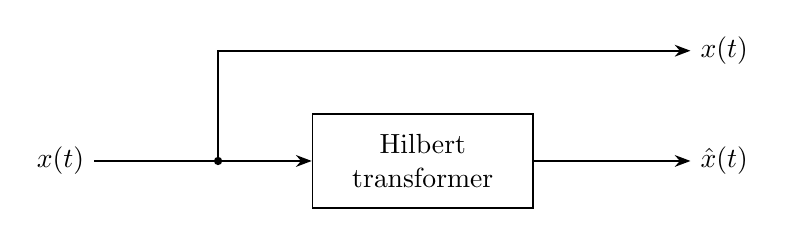
\begin{tikzpicture}[>=Stealth, line width=0.6pt]
    % 输入信号
    \node (in) at (0,0) {$x(t)$};
    % 分支点
    \coordinate (split) at (2,0);
    % Hilbert 变换器方框
    \node[draw, minimum width=2.8cm, minimum height=1.2cm, align=center]
         (ht) at (4.6,0) {Hilbert\\transformer};
    % 输出端
    \node[anchor=west] (out2) at (8,0)   {$\hat{x}(t)$};
    \node[anchor=west] (out1) at (8,1.4) {$x(t)$};

    % 连线
    \draw (in.east) -- (split);
    \draw[->] (split) -- (ht.west);
    \draw[->] (ht.east) -- (out2.west);
    \draw[->] (split) |- (out1.west);

    % 分支点实心圆
    \fill (split) circle (1.5pt);
  \end{tikzpicture}
  \caption{Generation of an analytic signal using a Hilbert transformer.}
\end{figure}

\end{document}
